\documentclass[a4paper, 12pt]{article}
\usepackage{config}

\usepackage{import}

\begin{document}
	\section{Introdução}
	
	Ao estudar as diferentes propriedades dos materiais biológicos, nos deparamos com questões fundamentais de serem estudas. As mesmas pode
	
	\section{Objetivo}
	
	Determinação do Módulo de Elasticidade (Módulo de Young).
	
	\section{Materiais e Métodos}
	
	Os seguintes materiais foram empregados no experimento:
	
	\begin{enumerate}
		\item Batata Inglesa;
		\item Cortador de batata cilíndrico;
		\item Paquímetro digital;
		\item Máquina Universal de Ensaios;
		\item Software para aquisição de dados.
	\end{enumerate}
	
	\import{sections/tables}{data}
	
	\section{Resultados e discussão}
	
	A partir dos gráficos obtidos, nota-se que ao elevar a velocidade de deformação dos corpos de prova cilíndricos ocorre elevação nos valores de módulo de elasticidade. Na primeira parte do experimento, sob velocidade de \SI{.5}{\milli\meter/\second}, foi obtido um valor de $\textrm{E}_{1}=\SI{3.22}{\mega\pascal}$ com base no ajuste realizado. Na segunda etapa, a \SI{.8}{\milli\meter/\second} o comportamento mecânico da batata inglesa ocasionou aumento de \SI{.32}{\mega\pascal} ($\textrm{E}_{2}=\SI{3.54}{\mega\pascal}$) e, por fim, na bateria final ($v_{3}=\SI{1.2}{\milli\meter/\second}$), o valor de $\textrm{E}$ foi novamente incrementado levando a um $\textrm{E}_{3}=\SI{3.77}{\mega\pascal}$. 
	
	\begin{figure}[h!]
		\centering
		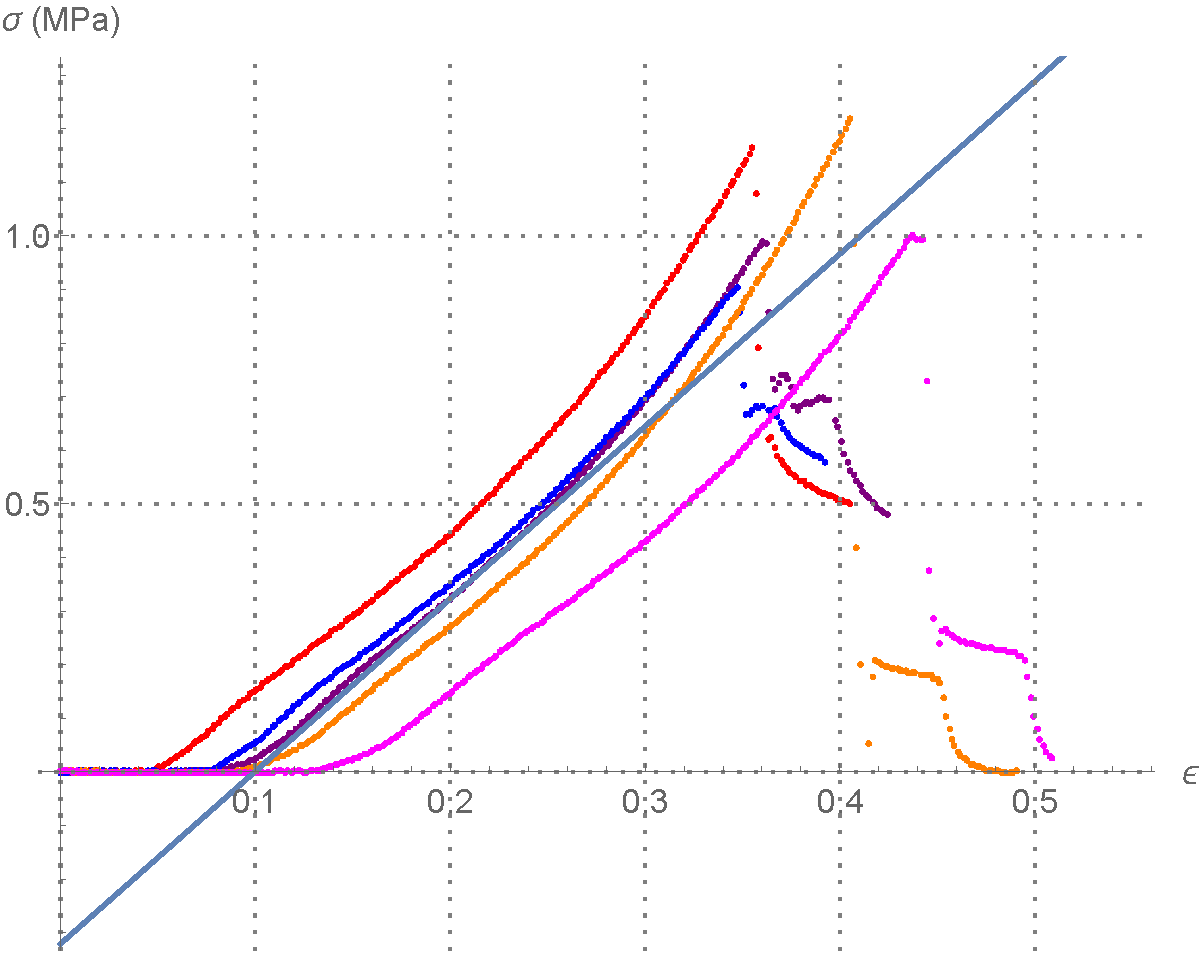
\includegraphics[width=0.7\linewidth]{sections/images/g1}
		\caption{Gráfico da tensão ($\sigma$, em \SI{}{\mega\pascal}) em função da deformação ($\epsilon$) sob compressão a \SI{.5}{\milli\meter/\second}}
		\label{fig:g1}
	\end{figure}
	
	\begin{figure}[h!]
		\centering
		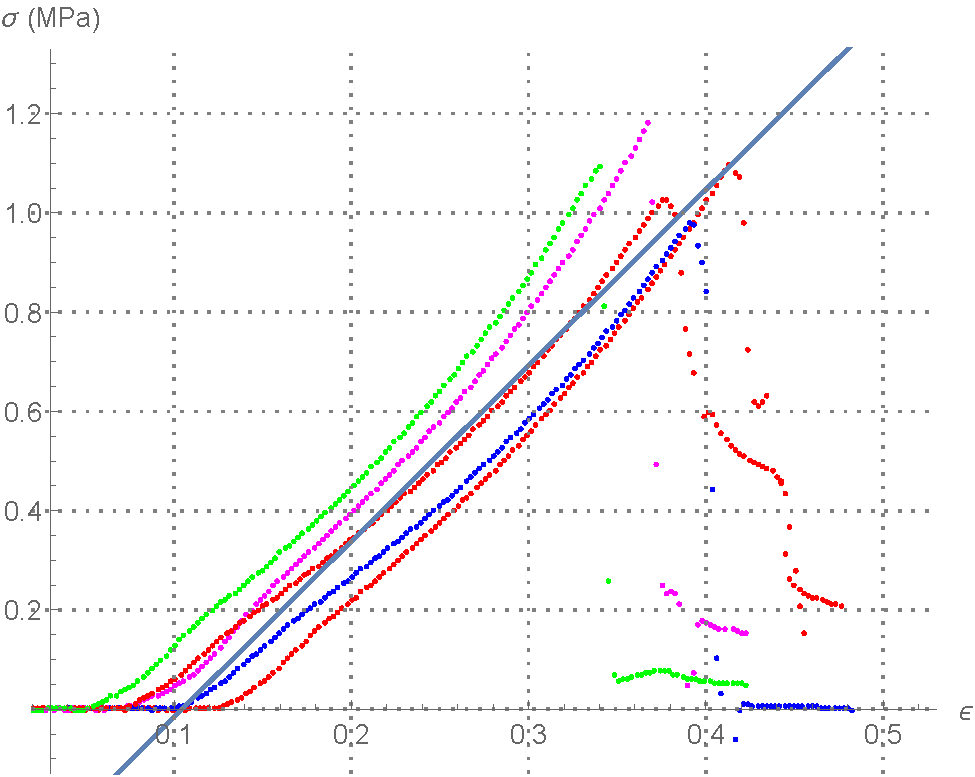
\includegraphics[width=0.7\linewidth]{sections/images/g2}
		\caption{Gráfico da tensão ($\sigma$, em \SI{}{\mega\pascal}) em função da deformação ($\epsilon$) sob compressão a \SI{.8}{\milli\meter/\second}}
		\label{fig:g2}
	\end{figure}

	\begin{figure}[h!]
		\centering
		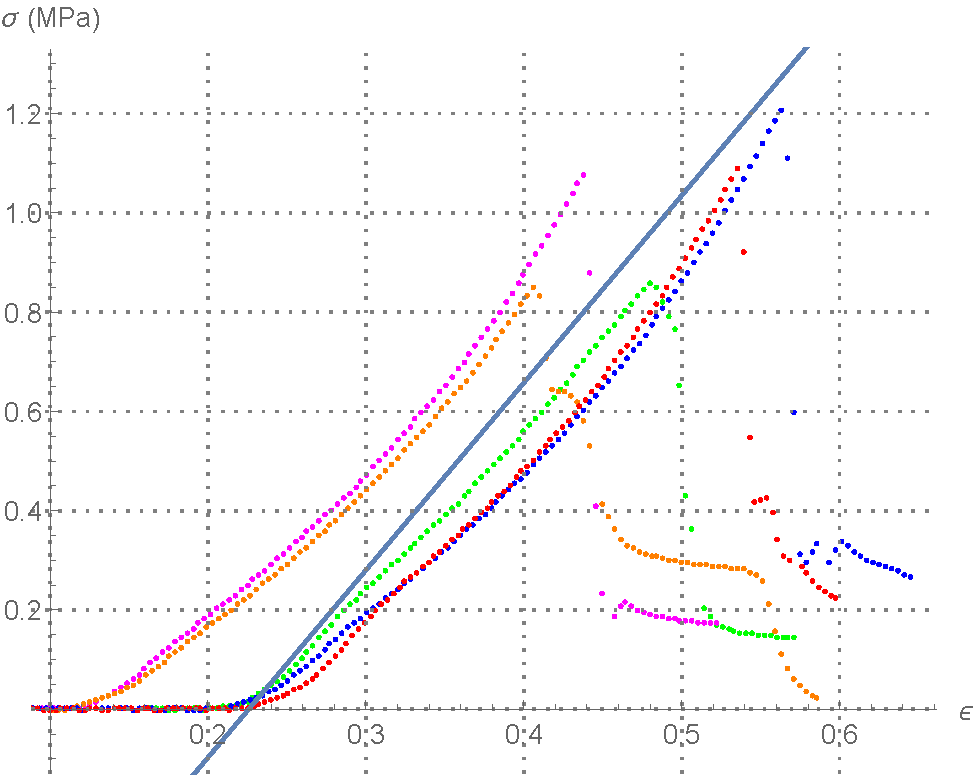
\includegraphics[width=0.7\linewidth]{sections/images/g3}
		\caption{Gráfico da tensão ($\sigma$, em \SI{}{\mega\pascal}) em função da deformação ($\epsilon$) sob compressão a \SI{1.2}{\milli\meter/\second}}
		\label{fig:g3}
	\end{figure}

	\begin{figure}[h!]
		\centering
		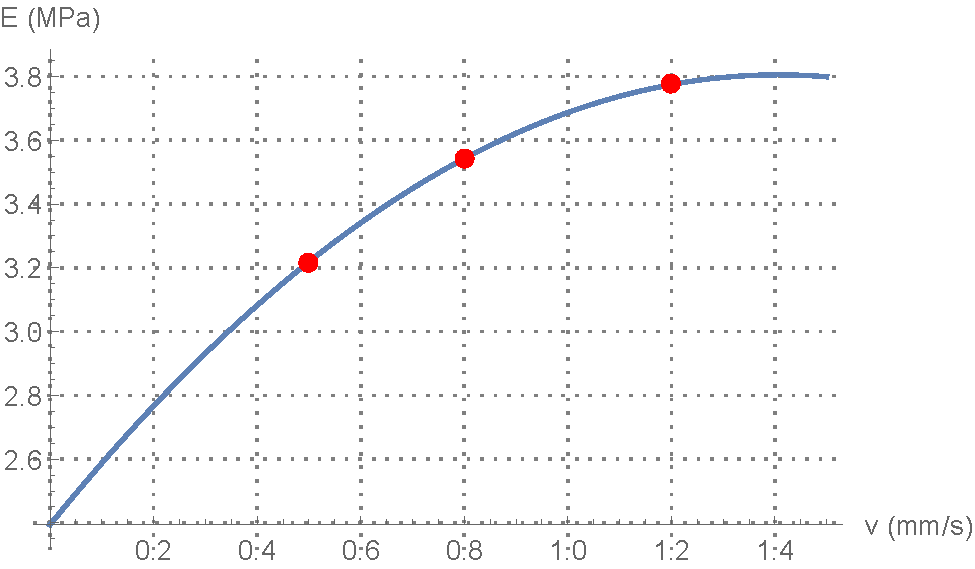
\includegraphics[width=0.7\linewidth]{sections/images/g4}
		\caption{Comportamento do módulo de elasticidade médio do corpo de prova sob diferentes velocidades na compressão.}
		\label{fig:g4}
	\end{figure}
	
	\section{Conclusão}

\end{document}